\documentclass[10pt,a4paper]{article}
\usepackage[margin=1.7cm]{geometry}
\usepackage[T1]{fontenc}
\usepackage{lmodern}
\usepackage{amsmath}
\usepackage{graphicx}
\usepackage{booktabs}
\usepackage{xcolor}
\usepackage{hyperref}
\usepackage{caption}
\usepackage{subcaption}
\usepackage{enumitem}
\usepackage{titlesec}
\usepackage{cleveref}
\usepackage{float}


\graphicspath{{../figures/template/}}
\setlist{nosep, leftmargin=*}
\titlespacing*{\section}{0pt}{4pt}{2pt}
\titlespacing*{\subsection}{0pt}{2pt}{1pt}
\titleformat{\section}{\normalsize\bfseries}{\thesection}{0.6em}{}
\setlength{\parskip}{2pt}
\setlength{\parindent}{0pt}
\captionsetup{font=small}
\captionsetup[table]{skip=3pt}
\setlength{\textfloatsep}{6pt plus 2pt minus 2pt}
\setlength{\intextsep}{6pt plus 2pt minus 2pt}
\newcommand{\fig}[1]{Fig.~\ref{fig:#1}}
\newcommand{\code}[1]{\texttt{#1}}

\begin{document}

\begin{center}
  {\large\bfseries Assignment 01 --- Walking while carrying a tray with TSID}\\[2pt]
  Optimization and Learning for Robot Control, University of Trento\\[2pt]
  Daniele Trisotto (267254), \quad Michele Macellari (267255)
\end{center}

All figures and indicators are produced from the repository root with
\begin{center}
  \colorbox{gray!12}{\strut\enspace\texttt{python3 template\_figures.py q1}\quad\textcolor{gray}{\# or q2, q3, q4, q5, all}\enspace}
\end{center}
which runs the templates with the parameters of each question (no viewer, default \code{romeo\_conf.py} plus the listed overrides).

\section{Walking with double support}
\textbf{Weight Transfer.} In single support the stance foot carries the whole weight and the swing foot 0\,N (\fig{q1ds}). The reference CoP stays under the stance foot ($y=\pm0.096$\,m) and. Without DS the CoP jumps by 19.2\,cm in one 2\,ms step and the whole weight is transferred in one step (\fig{q1ds}). With a single contact the CoP must stay inside that sole, so without a phase with two contacts it can only jump. Hence, the max normal force change rate is 11 times larger without DS (195\,kN/s vs 17.8\,kN/s) and so is that of the joint torque (28.8 vs 6.3\,kNm/s).

\textbf{Real Robot.} Without DS the walk works only because the simulation is ideal: the state is integrated from the QP accelerations, contacts are rigid and instantaneous and the touchdown time is exact. On a real robot torques cannot change in 2\,ms (actuator bandwidth), the swing foot would take the whole weight during the impact, an early/late touchdown (model errors, uneven ground) would transfer the weight to a foot not yet on the ground, and noisy, delayed force sensors cannot confirm the contact so quickly.

\textbf{Fall with \code{transition\_time = 0.1} and Fix.} \code{removeRigidContact(name, 0.1)} keeps the contact for 0.1\,s while decreasing linearly its maximum normal force $f_{max}$ to 0, then removes it; the ramp leaves $f_{max}=0$ inside the \code{Contact6d}, and \code{addRigidContact} re-adds the same object without restoring it. In \fig{q1fall} the left foot is removed at the start ($f_{max}^{LF}\to0$ at 1.4\,s); at touchdown (2.5\,s) the constraint $0\le f_N\le f_{max}=0$ forbids it to carry any load, so when the right foot is lifted the robot falls (2.81\,s). Fix: \code{contactRF/LF.setMaxNormalForce(conf.fMax)} in \code{add\_contact\_RF/LF} before \code{addRigidContact}; the walk is then completed (\fig{q1fixed}). The ramp makes only little difference with this gait: same CoM error (2.9/6.8\,mm RMS/max), force rate $17.8\to15.0$\,kN/s, torque rate $6.3\to4.6$\,kNm/s. The weight is already transferred by the DS through the CoP: when the ramp starts (2.6\,s) the actual force is already below it, so it is active only in the last $\approx$20\,ms. (Without DS the ramp makes the robot fall even with the fix: the only stance foot would be unloaded.)

\begin{table}[H]
  \centering\small
  \begin{tabular}{lccc}
    \toprule
    Configuration         & CoM Error RMS/Max & Max $\dot{F}_n$ & Max $\dot{\tau}$ \\
    \midrule
    DS                    & 2.9/6.8\,mm       & 17.8\,kN/s      & 6.3\,kNm/s       \\
    NoDS                  & 2.2/5.3\,mm       & 195.2\,kN/s     & 28.8\,kNm/s      \\
    DS, $T_{tr} = 0.1$\,s & 2.9/6.8\,mm       & 15.0\,kN/s      & 4.6\,kNm/s       \\
    \bottomrule
  \end{tabular}
  \caption{Q1, CoM error and maximum rate of change of normal forces and torques ($T_{tr}$ = \code{transition\_time}, 0 if not shown; with the fix).}
  \label{table:Q1}
\end{table}

\section{Tray along a sinusoid}
Hand task: \code{TaskSE3Equality}, $K_p=10$, $K_d=2\sqrt{K_p}$, mask and frame from the conf, added only if \code{w\_hand>0.0} or \code{hand\_priority = 0}. Reference: $p=c+A\sin\omega t$, $\dot p = A\omega\cos\omega t$, $\ddot p=-A\omega^2\sin\omega t$.

\textbf{Without Feedforward.} $\dot p^{ref}=\ddot p^{ref}=0$ and only $\ddot p^d = K_p(p^{ref}-p)-K_d\dot p$ is left: the hand moves only because of the position error, so it lags behind and moves less. It is a critically damped low-pass filter $P/P^{ref}=K_p/(s^2+K_ds+K_p)$ with $\omega_n=\sqrt{K_p}\approx0.5$\,Hz: at 0.5\,Hz ($=\omega_n$) theory gives 0.50/89.6$^\circ$, at 2\,Hz ($\approx4\omega_n$, attenuation $\propto K_p/\omega^2$) 0.06/151.8$^\circ$; the simulated values (\Cref{table:Q2}) match the theory (\fig{q2track}).

\textbf{With Feedforward.} Ideally $\ddot e+K_d\dot e+K_pe=0$ (perfect tracking, $e = p^{ref}-p$): the lag is indeed small ($\le10^\circ$) but the amplitude drops at high frequency. The reason is the CoM: the base is floating, so accelerating the arm and tray pushes the rest of the body and moves the CoM, while the CoM task, with the same weight ($w_{com}=w_{hand}=1$), wants to keep it still; the QP compromises. The required acceleration $A\omega^2$ is 16 times larger at 2\,Hz (7.9 vs 0.49\,m/s$^2$): the CoM moves by 5.5\,cm (vs 7\,mm) and drifts, the hand oscillates around a lower height, and the right ankle reaches its torque limit (\fig{q2com}, \fig{q2track}).

\begin{table}[H]
  \begin{center}\small
    \begin{tabular}{lcccc}
      \toprule
      Result                      & 0.5\,Hz, FF        & 0.5\,Hz, NoFF       & 2\,Hz, FF          & 2\,Hz, NoFF          \\
      \midrule
      Amplitude Ratio / Phase Lag & 0.87 / 8.1$^\circ$ & 0.44 / 97.2$^\circ$ & 0.43 / 7.7$^\circ$ & 0.05 / 156.5$^\circ$ \\
      Max CoM Displacement        & 7.3\,mm            & 3.6\,mm             & 54.7\,mm           & 0.9\,mm              \\
      \bottomrule
    \end{tabular}
  \end{center}
  \caption{Q2, Amplitude ratio/phase lag and CoM displacement for different frequency (0.5\,Hz, 2\,Hz) with and without feedforward (FF/NoFF).}
  \label{table:Q2}
\end{table}

\section{Walking with the tray}
Hand reference: initial height and orientation, $x$/$y$ = initial hand position + displacement of the CoM reference, velocity/acceleration = those of the CoM reference (zero along $z$). \Cref{table:Q3} compares the walk without and with the hand task: the tray stays horizontal and the hand follows its reference, but the CoM tracking gets worse, mostly along $y$ (\fig{q3hand}, \fig{q3com}). The cause is not the mass of the arm but the kinematic coupling: the hand pose depends on legs, pelvis and torso, the same DOFs used by the CoM task. Walking makes the body sway ($\pm8$\,cm laterally) and, without the hand task, this sway is transferred to the tray; keeping the hand still requires counteracting the upper-body motion, which also moves the CoM. With equal weights the QP sacrifices part of the CoM tracking, and the 6D hand task leaves less redundancy to the CoM task.

\begin{table}[H]
  \centering\small
  \begin{tabular}{lcccc}
    \toprule
    Hand Weight          & Max Tilt      & Max Hand Error & CoM Error RMS/Max \\
    \midrule
    \code{w\_hand = 0.0} & 12.75$^\circ$ & 66.2\,mm       & 2.9/6.8\,mm       \\
    \code{w\_hand = 1.0} & 0.04$^\circ$  & 8.8\,mm        & 7.1/14.4\,mm      \\
    \bottomrule
  \end{tabular}
  \caption{Q3, Max tilt and errors of hand and CoM with hand task on and off.}
  \label{table:Q3}
\end{table}

\section{Mask and frame of the tray task}

Results in \Cref{table:Q4} and \fig{q4time}. Position only: the orientation is free and the tray tilts up to 22$^\circ$. Attitude only: the tray is horizontal but the hand moves by 86\,mm with the body. The waiter needs constant height and no rotation about the horizontal axes, while $x$, $y$ and the yaw angle are free, leading to the mask $[0,0,1,1,1,0]$, a requirement defined in the \emph{world} frame. In the world-aligned frame the mask selects exactly height and tilt: the requirement is met as with the full mask (0.03$^\circ$, 10.5\,mm) with half the CoM error (3.6 vs 7.1\,mm), since only 3 DOFs are constrained. In the local frame the same mask selects components along the hand axes, which are not aligned with the world (the hand $z$ axis is 53$^\circ$ from the vertical) and rotate with the hand: freeing $r_z$ frees part of the tilt and freeing $x$-$y$ frees part of the vertical motion (8.9$^\circ$, 78\,mm). With the full mask the frame is irrelevant (identical results): the error is the same vector in different axes and, with equal gains, its norm does not change.

\begin{table}[H]
  \begin{center}\small
    \begin{tabular}{lccc}
      \toprule
      $[x,y,z,r_x,r_y,r_z]$ Mask Type, Frame & Max Tilt      & Height Range & CoM RMS \\
      \midrule
      $[1,1,1,1,1,1]$ Pose, Local            & 0.04$^\circ$  & 13.5\,mm     & 7.1\,mm \\
      $[1,1,1,0,0,0]$ Position, Local        & 21.88$^\circ$ & 14.1\,mm     & 5.3\,mm \\
      $[0,0,0,1,1,1]$ Attitude, Local        & 0.02$^\circ$  & 85.5\,mm     & 3.1\,mm \\
      $[0,0,1,1,1,0]$ Waiter, Local          & 8.89$^\circ$  & 78.4\,mm     & 3.9\,mm \\
      $[0,0,1,1,1,0]$ Waiter, World          & 0.03$^\circ$  & 10.5\,mm     & 3.6\,mm \\
      \bottomrule
    \end{tabular}
  \end{center}
  \caption{Q4, results for the different hand masks and frames (the full mask gives identical results in the world-aligned frame).}
  \label{table:Q4}
\end{table}
\section{Heavy trays}
\textbf{5 kg Tray.} The robot shifts its pelvis by $\approx$3.5\,cm to the left and 2.3\,cm backwards for the whole walk (leaning away from the tray, which is in front-right of the pelvis), while the total CoM (robot + tray) is unchanged within a few mm (\fig{q5pelvis}). The payload is in the model, so the CoM task controls the CoM of robot + tray with the same reference; to compensate the 5\,kg at $\approx$0.31\,m to the right, the CoM of the robot alone moves by 2.7\,cm left and 1.8\,cm back, mainly by moving the pelvis. The hand task ($w_{hand}=100$) keeps the tray in place, so the posture task, with the lowest weight, gives way.

\textbf{2 kg Tray, Nominal Limits.} With the hand task as a hard constraint (\code{hand\_priority = 0}) the QP becomes infeasible at 2.23\,s, because it conflicts with the \textbf{torque bounds}, in particular of \code{RWristPitch}, the joint carrying the tray (limit $0.6\times1.45=0.87$\,Nm), already at 90\% when standing and at 100\% just before the failure (right knee at 91\%) (\fig{q5tau}, \fig{q5tray}). With $w_{hand}=100$ the walk is completed: the wrist stays at its limit for 1.24\,s and the QP sacrifices hand tracking instead (hand dropping by 13\,mm at each step, error up to 32\,mm vs 0.4\,mm with the empty tray, tilt 0.18$^\circ$) and slightly the CoM (8.5 vs 7.6\,mm RMS). Hard constraints should be used for what is physically mandatory and always satisfiable (dynamics, contacts, torque/joint limits): if two of them become incompatible the QP has no solution and the robot falls. Objectives that may conflict with the physics (hand pose, CoM, posture) should be weighted costs: a large weight gives almost strict priority when feasible but lets the task degrade gracefully when it is not.

\clearpage
\begin{figure}[p]\centering
  \begin{subfigure}{0.49\linewidth}\centering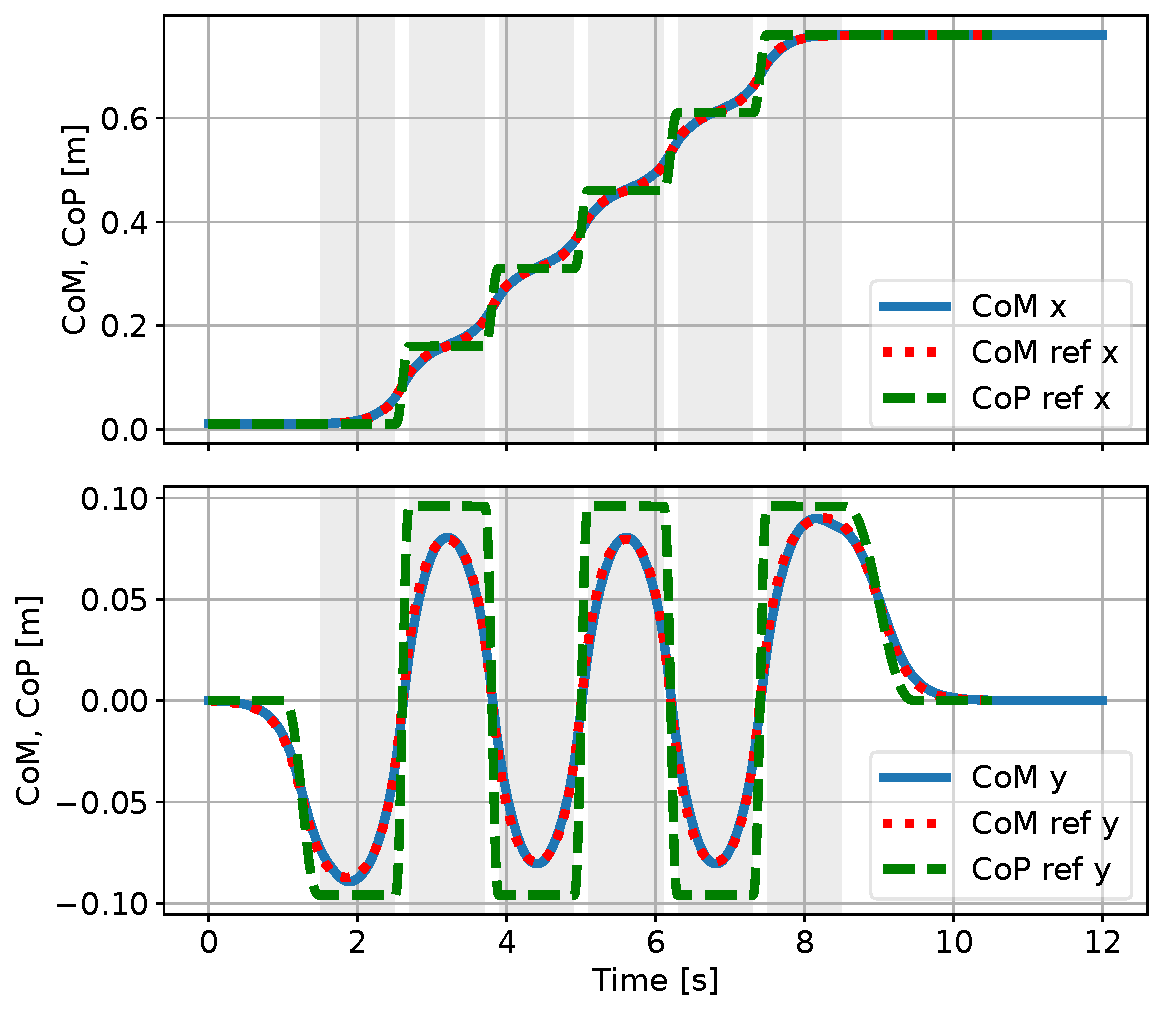
\includegraphics[width=\linewidth]{q1_ds_com}\caption{With DS: CoM, CoM ref., CoP ref.}\end{subfigure}
  \hfill
  \begin{subfigure}{0.49\linewidth}\centering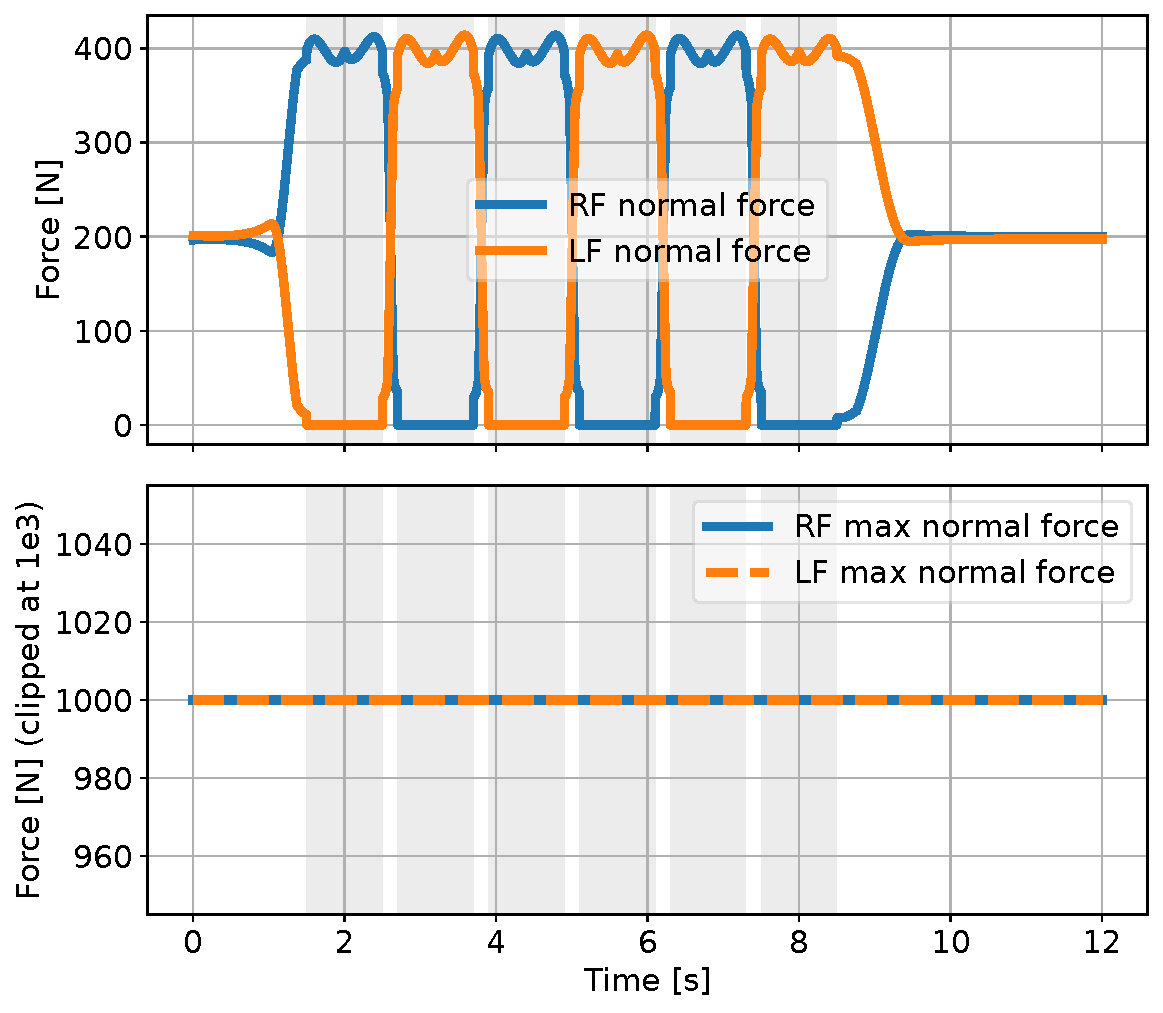
\includegraphics[width=\linewidth]{q1_ds_forces}\caption{With DS: normal forces and maximum normal forces}\end{subfigure}
  \medskip
  \begin{subfigure}{0.49\linewidth}\centering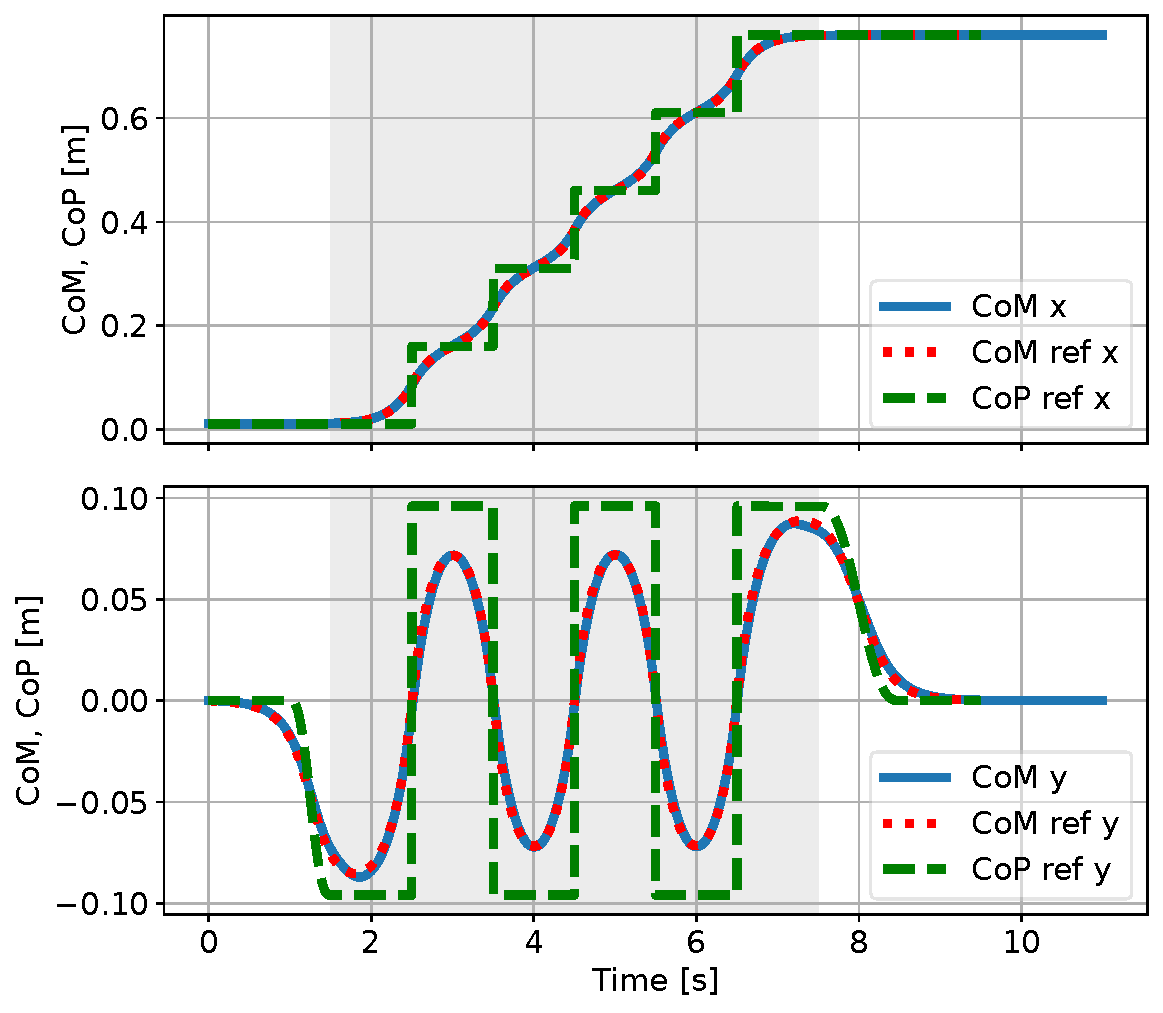
\includegraphics[width=\linewidth]{q1_nods_com}\caption{Without DS: CoM, CoM ref., CoP ref.}\end{subfigure}
  \hfill
  \begin{subfigure}{0.49\linewidth}\centering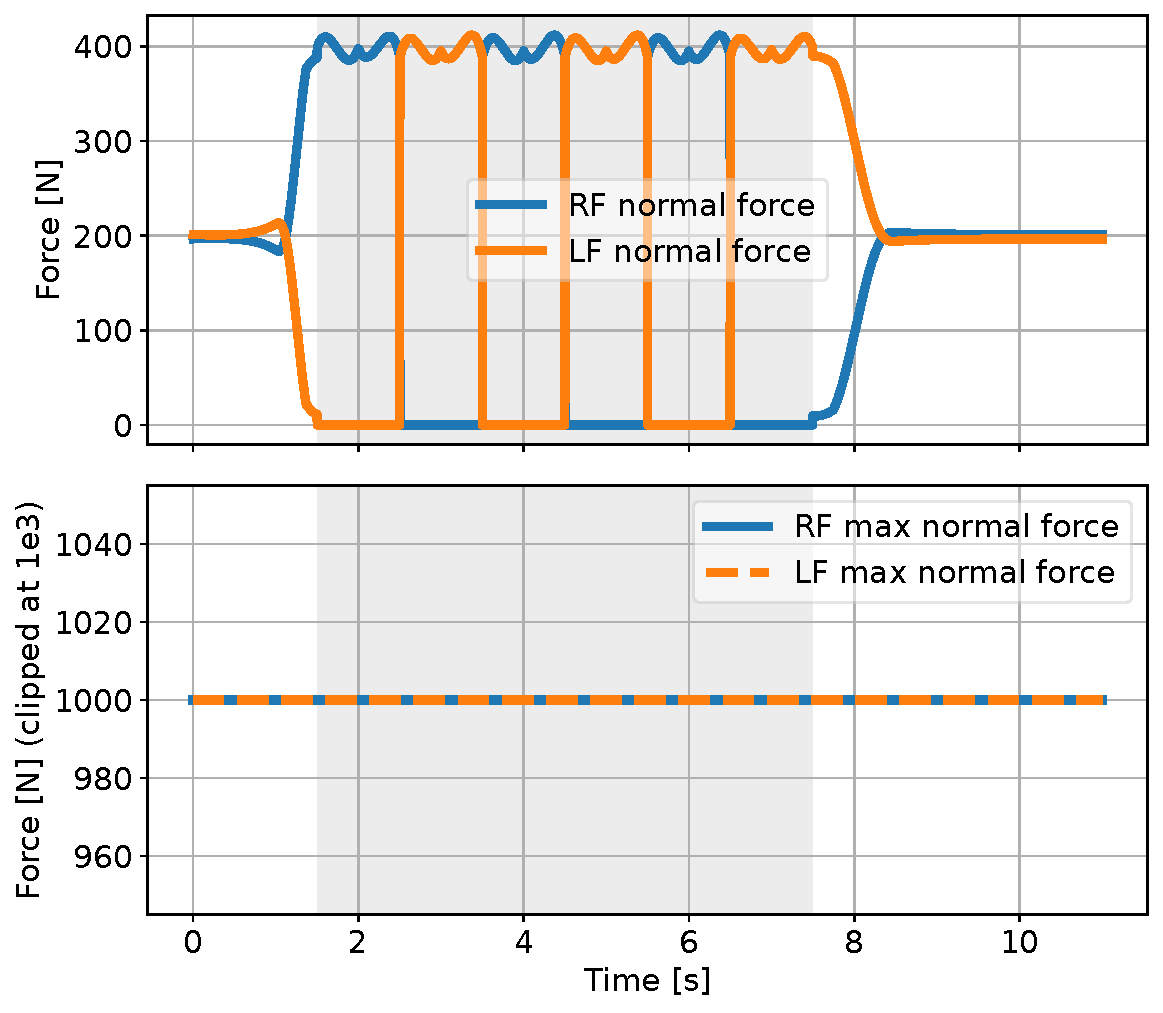
\includegraphics[width=\linewidth]{q1_nods_forces}\caption{Without DS: normal forces and maximum normal forces}\end{subfigure}
  \caption{Q1, Walk with and without double support (DS), \code{transition\_time = 0.0} (grey: single support).}\label{fig:q1ds}
\end{figure}

\begin{figure}[p]\centering
  \begin{subfigure}{0.49\linewidth}\centering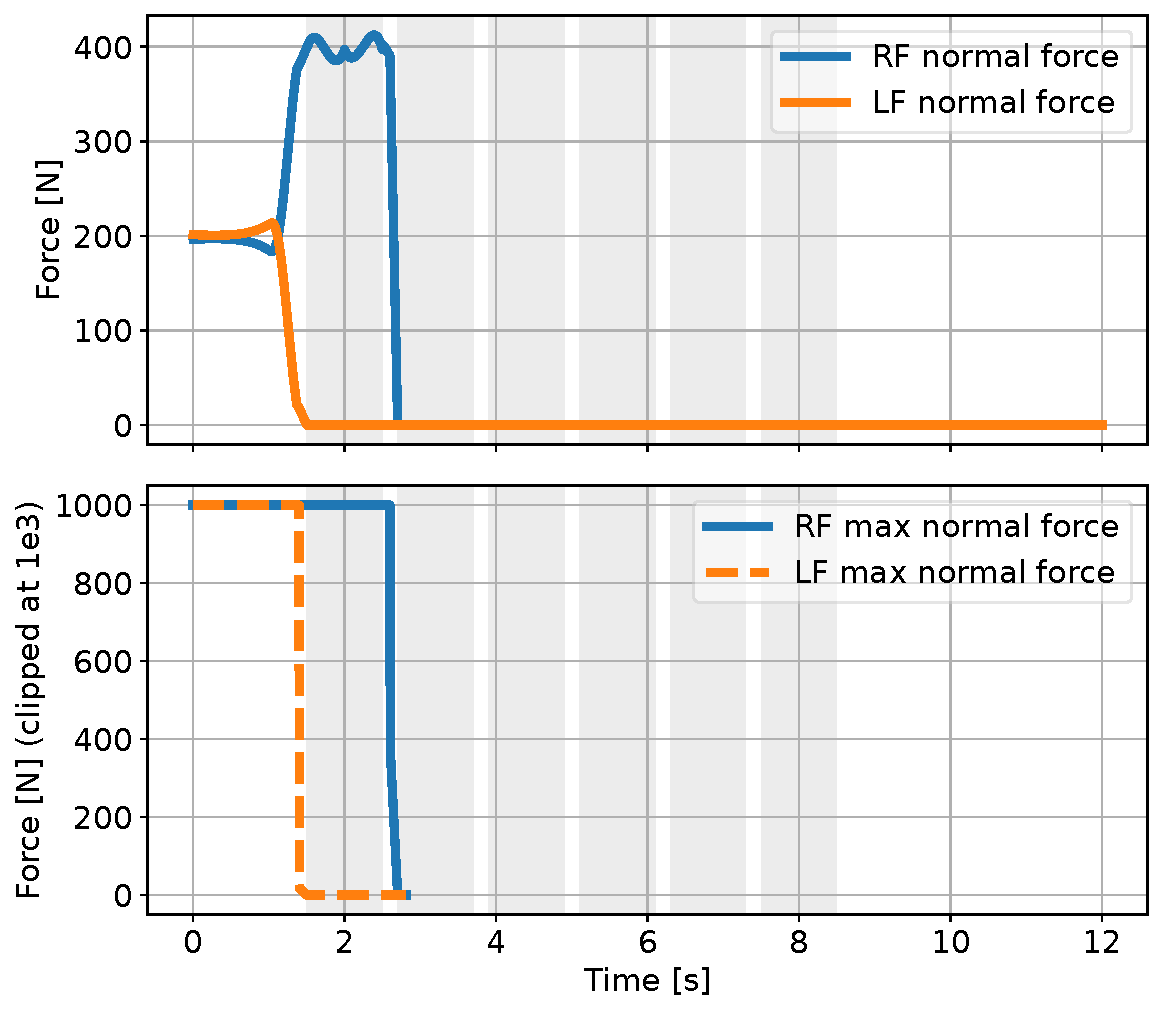
\includegraphics[width=\linewidth]{q1_fall_forces}\caption{Robot fall.}\label{fig:q1fall}\end{subfigure}
  \hfill
  \begin{subfigure}{0.49\linewidth}\centering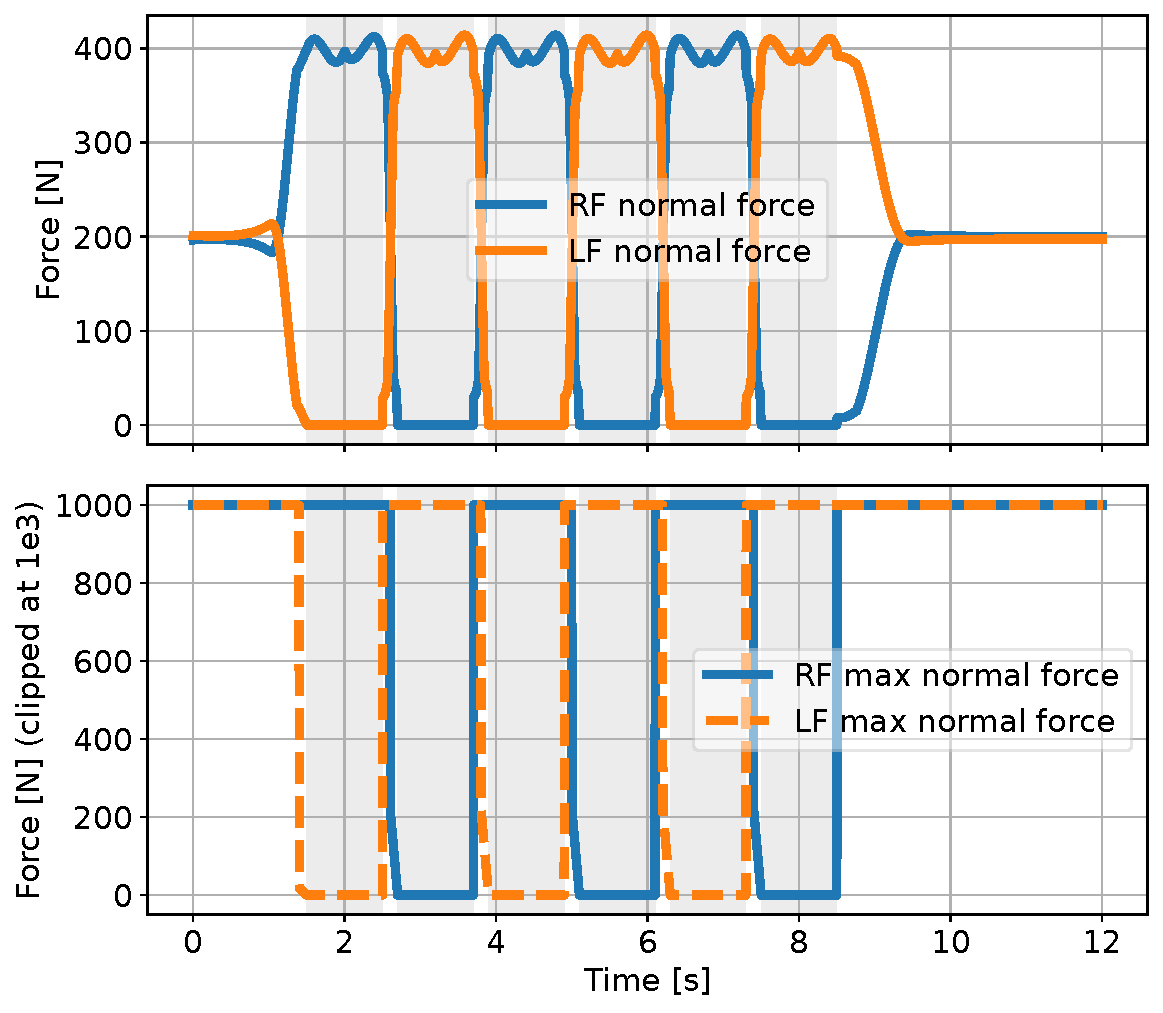
\includegraphics[width=\linewidth]{q1_fix_forces}\caption{Walk successfully completed.}\label{fig:q1fixed}\end{subfigure}
  \caption{Q1, \code{transition\_time = 0.1}: Normal forces and maximum normal forces of the feet.}
\end{figure}

\begin{figure}[p]\centering
  \begin{subfigure}{0.49\linewidth}\centering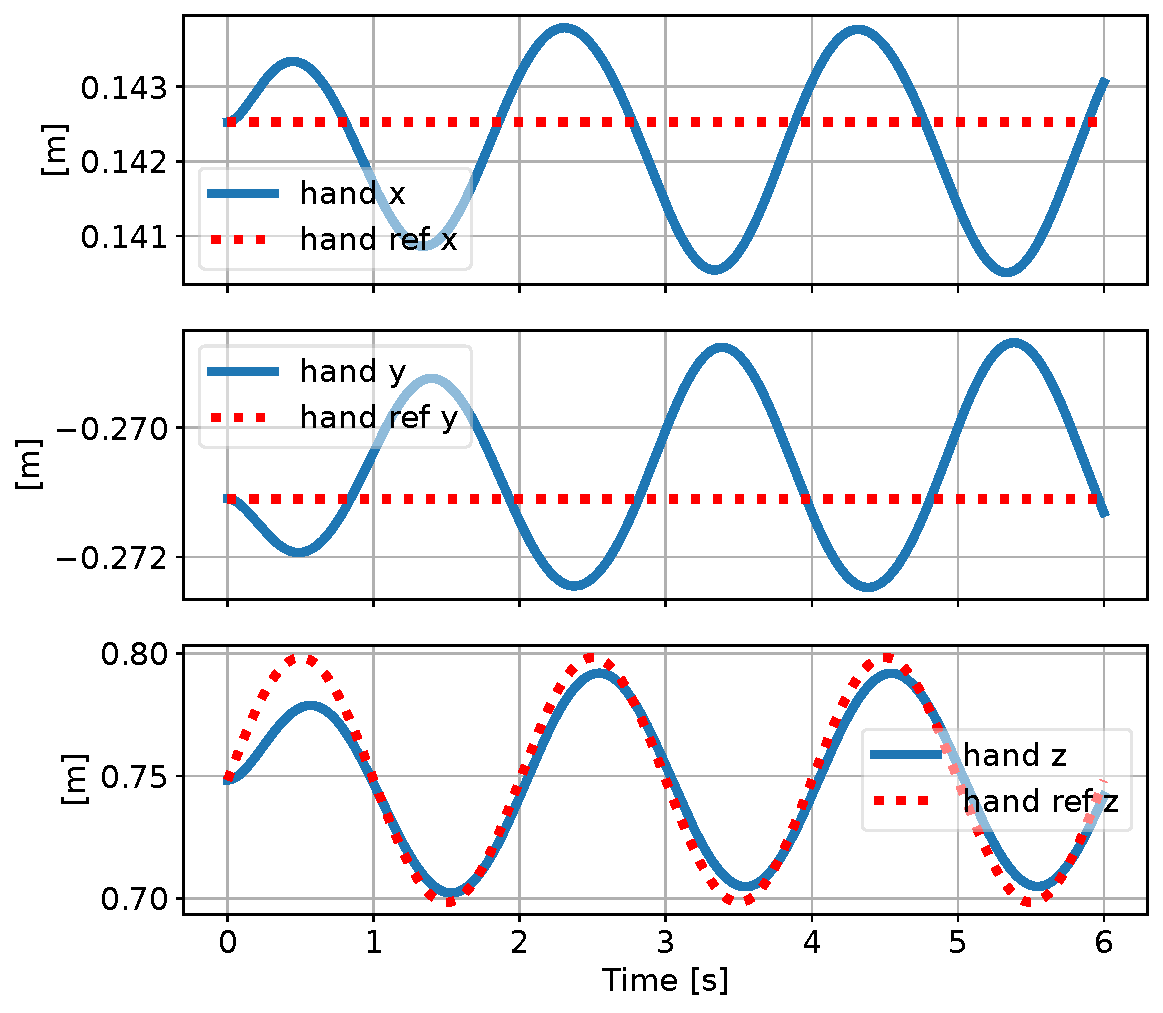
\includegraphics[width=\linewidth]{q2_0p5hz_ff_hand}\caption{0.5\,Hz, With feedforward}\end{subfigure}
  \hfill
  \begin{subfigure}{0.49\linewidth}\centering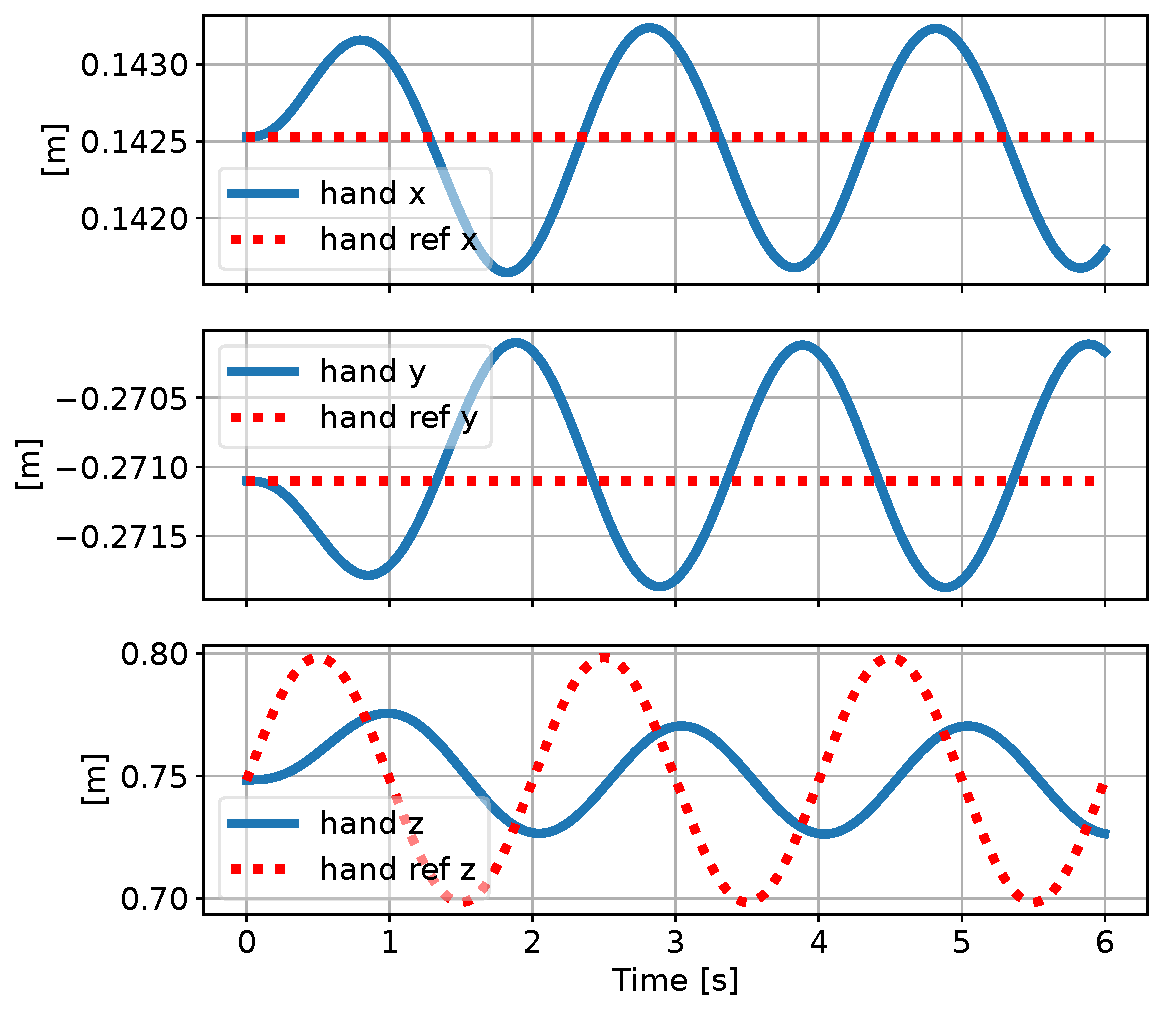
\includegraphics[width=\linewidth]{q2_0p5hz_noff_hand}\caption{0.5\,Hz, Without feedforward}\end{subfigure}
  \medskip
  \begin{subfigure}{0.49\linewidth}\centering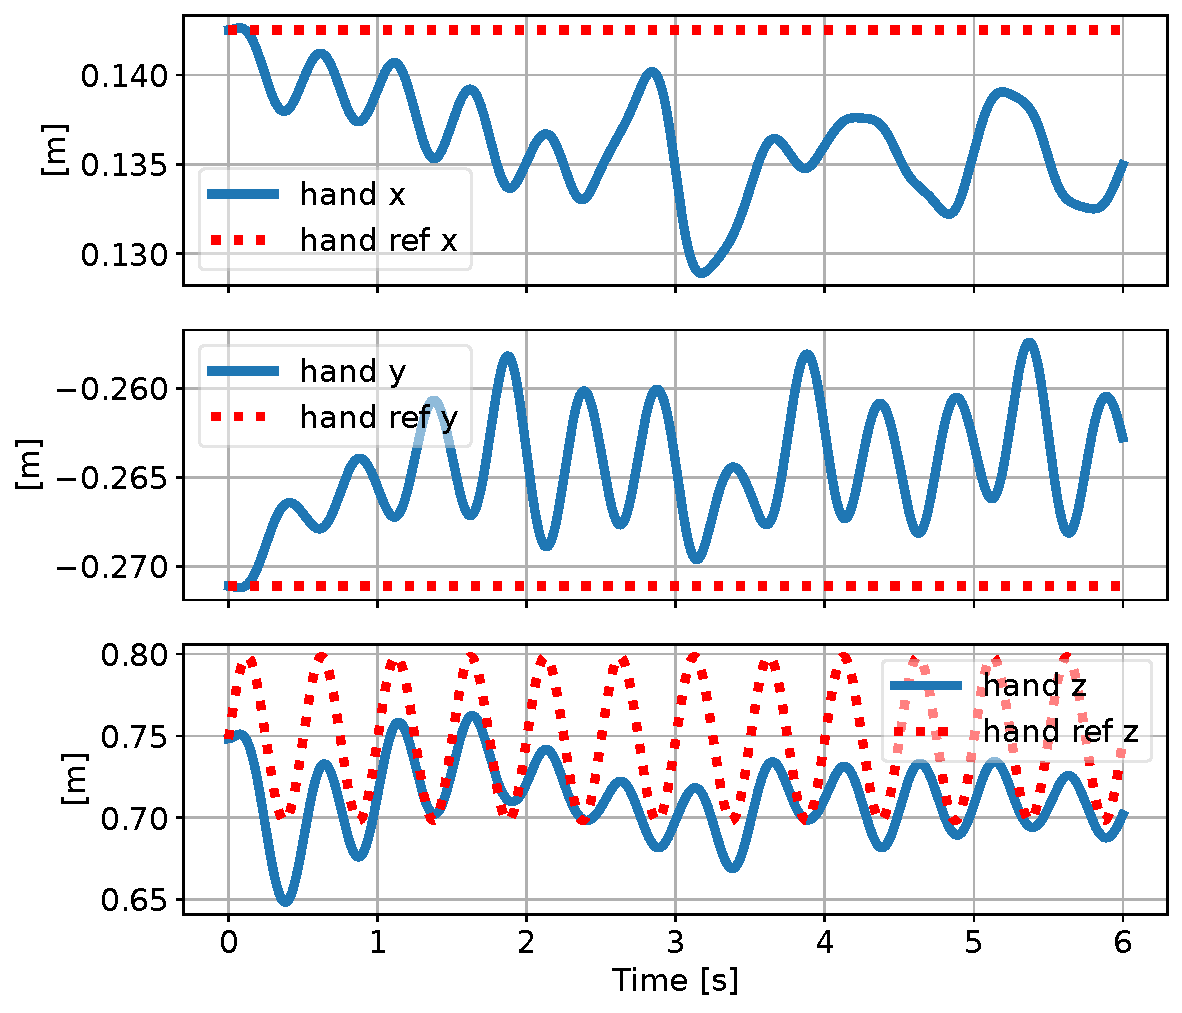
\includegraphics[width=\linewidth]{q2_2hz_ff_hand}\caption{2\,Hz, With feedforward}\end{subfigure}
  \hfill
  \begin{subfigure}{0.49\linewidth}\centering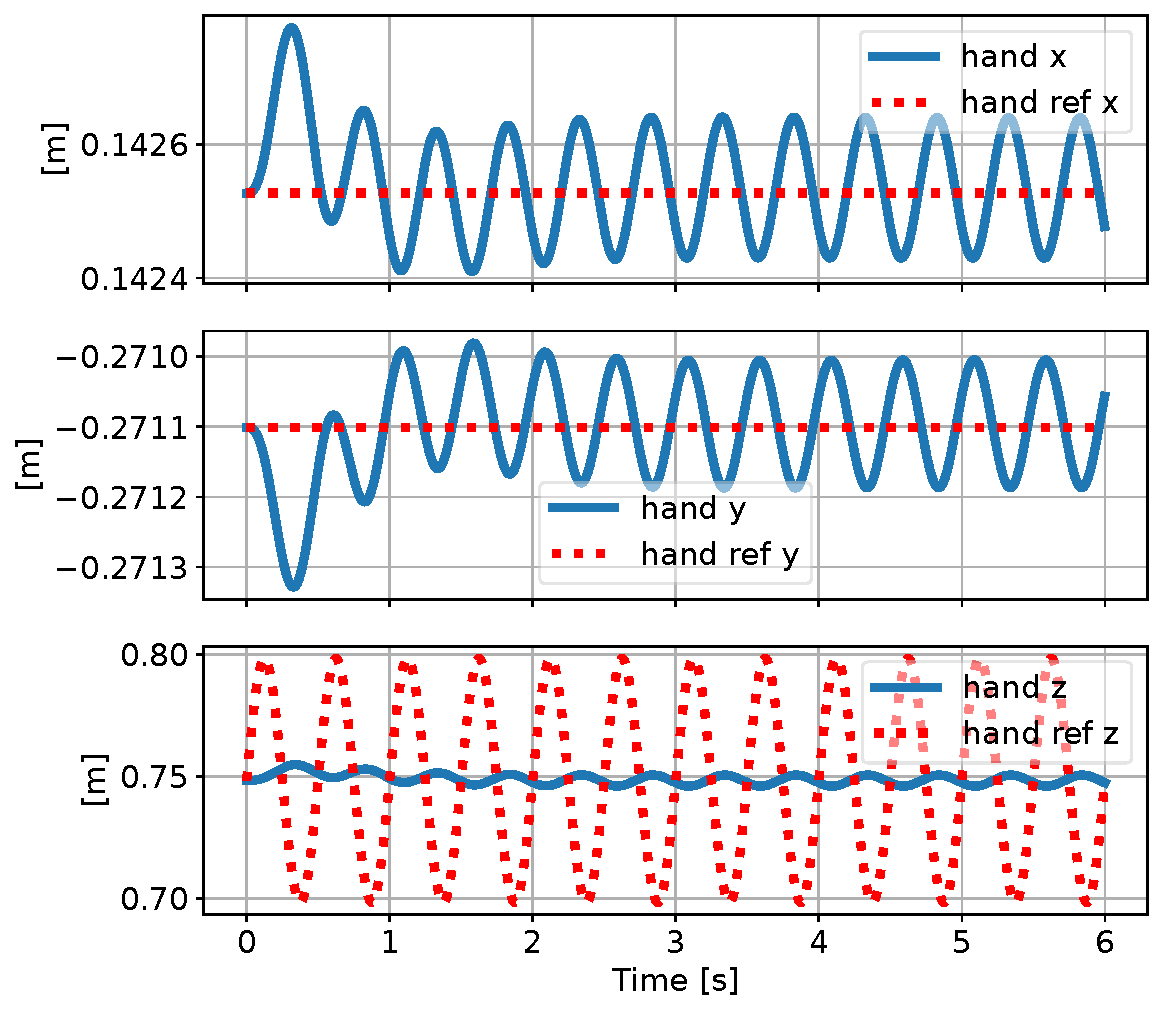
\includegraphics[width=\linewidth]{q2_2hz_noff_hand}\caption{2\,Hz, without feedforward}\end{subfigure}
  \caption{Q2, Hand position and reference along $x$, $y$, $z$.}\label{fig:q2track}
\end{figure}

\begin{figure}[p]\centering
  \begin{subfigure}{0.49\linewidth}\centering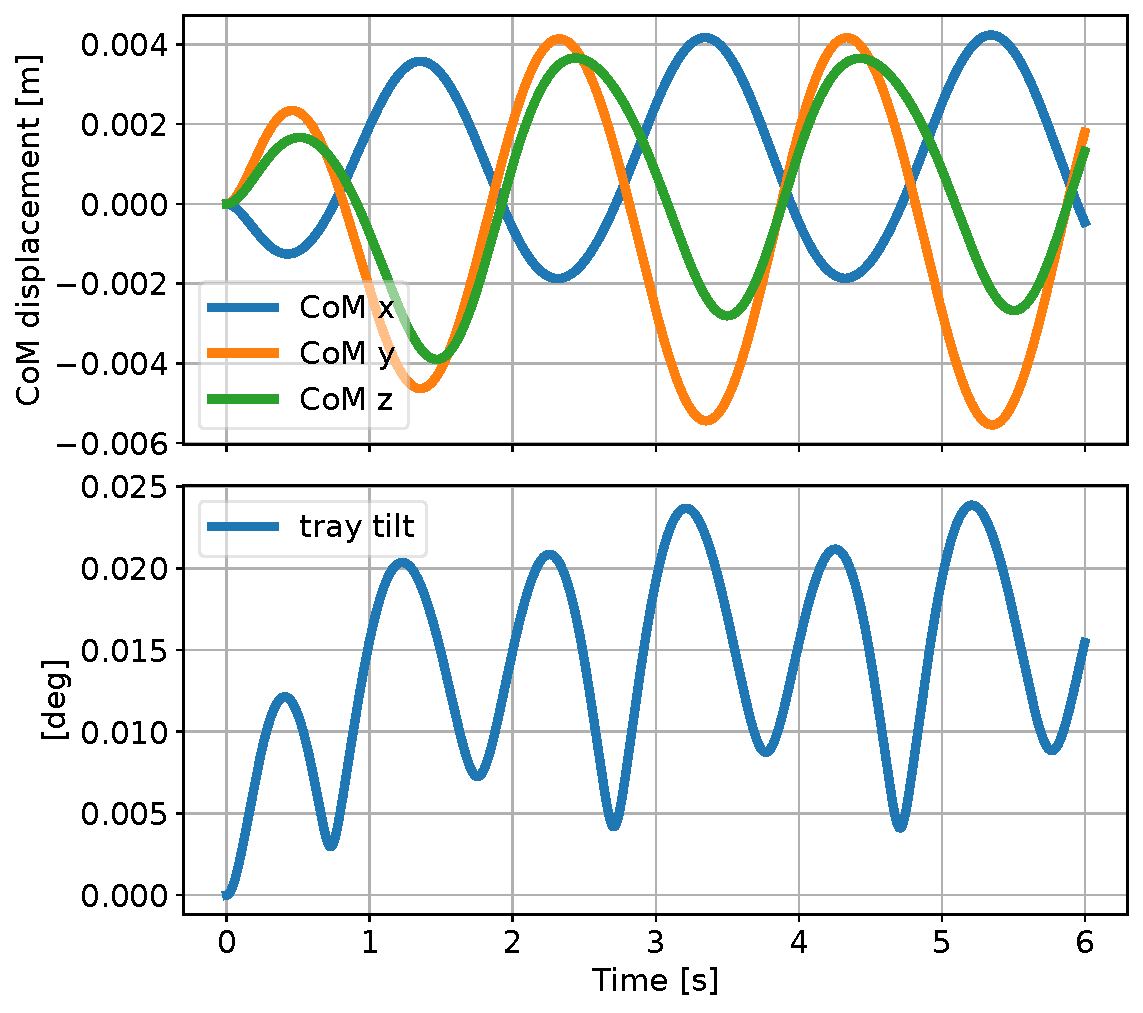
\includegraphics[width=\linewidth]{q2_0p5hz_ff_com}\caption{0.5\,Hz, With feedforward}\end{subfigure}
  \hfill
  \begin{subfigure}{0.49\linewidth}\centering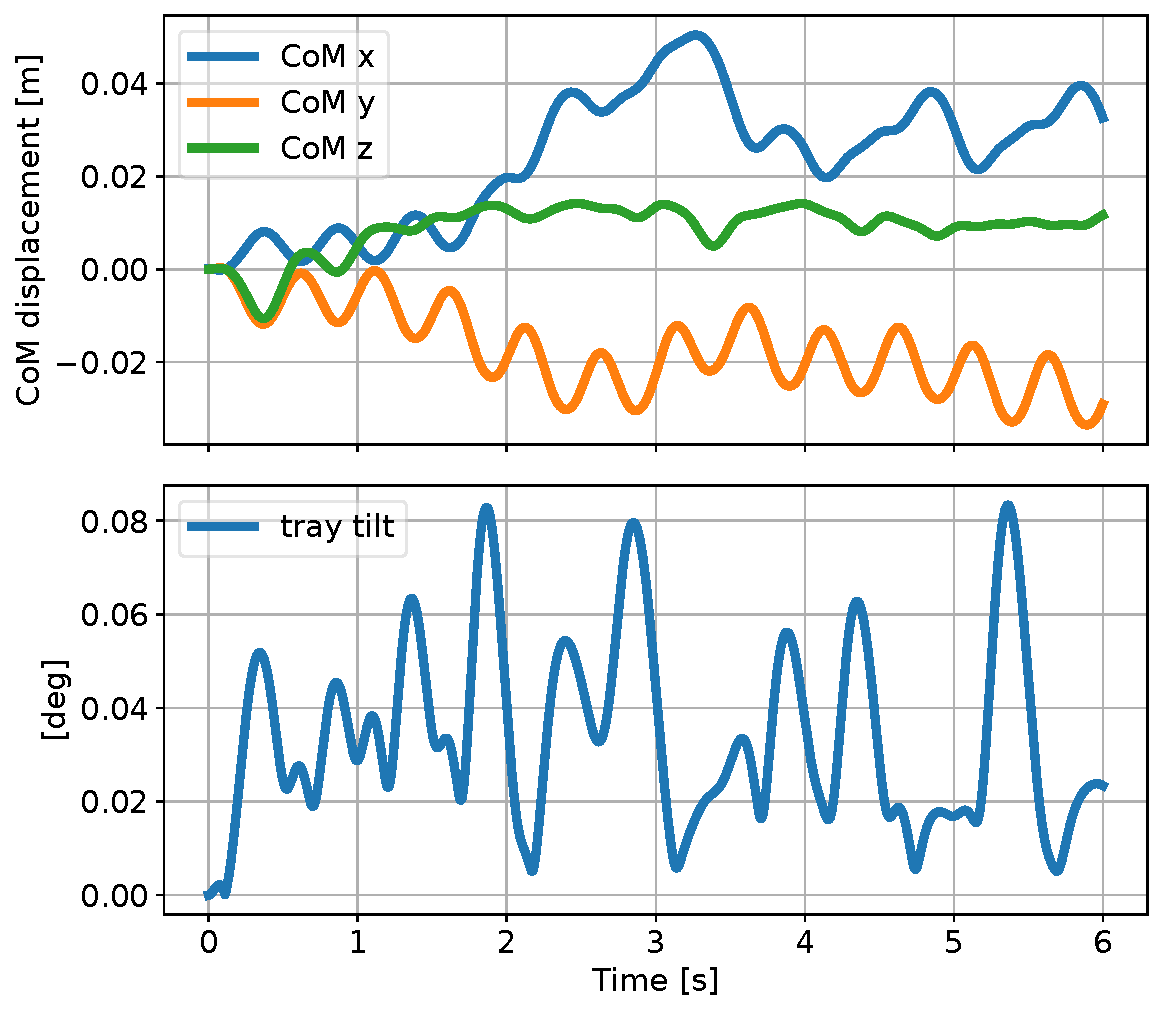
\includegraphics[width=\linewidth]{q2_2hz_ff_com}\caption{2\,Hz, With feedforward}\end{subfigure}
  \caption{Q2, CoM displacement and tray tilt with feedforward.}\label{fig:q2com}
\end{figure}

\begin{figure}[p]\centering
  \begin{subfigure}{0.49\linewidth}\centering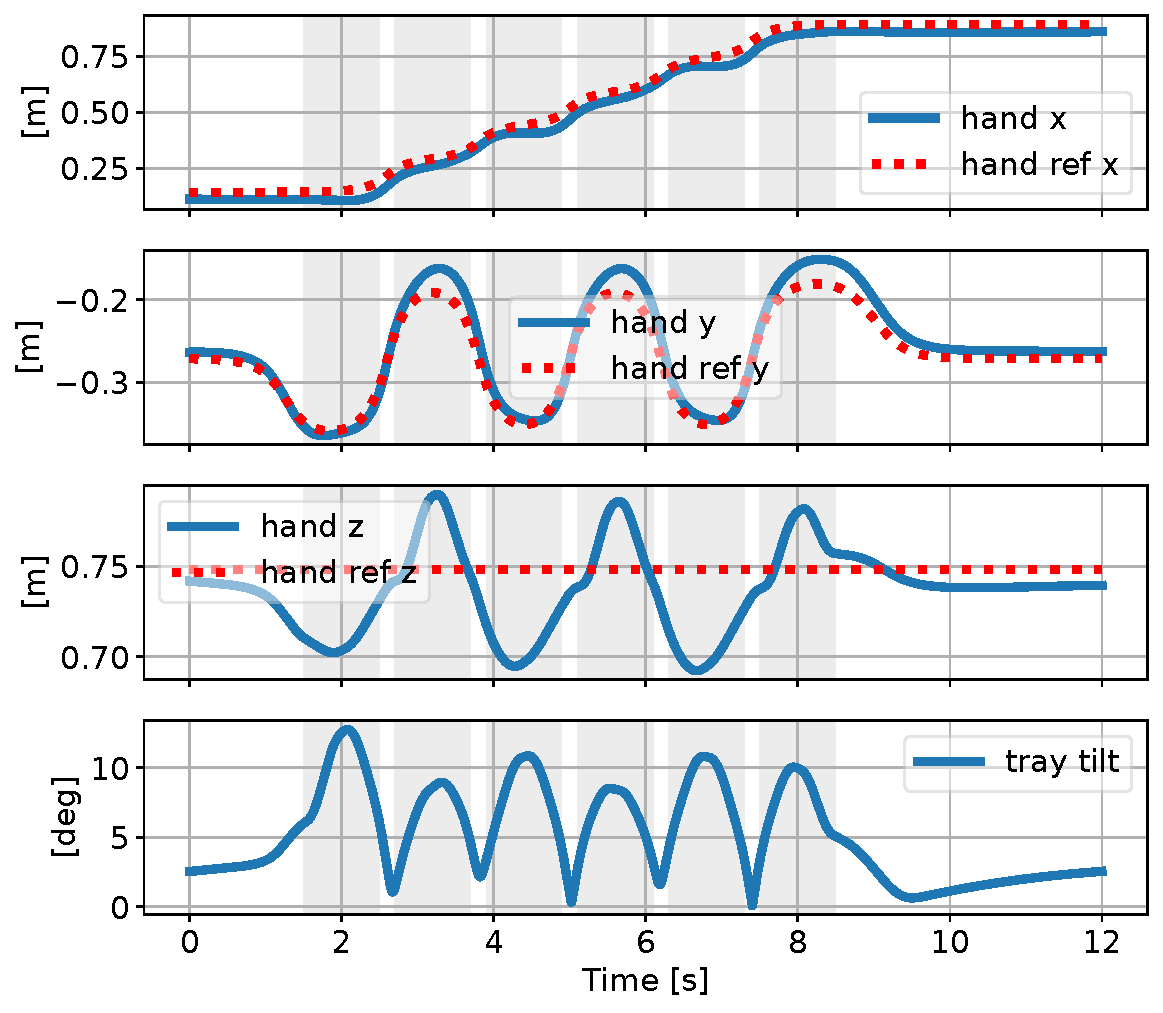
\includegraphics[width=\linewidth]{q3_whand0_hand}\caption{\code{w\_hand} = 0}\end{subfigure}
  \hfill
  \begin{subfigure}{0.49\linewidth}\centering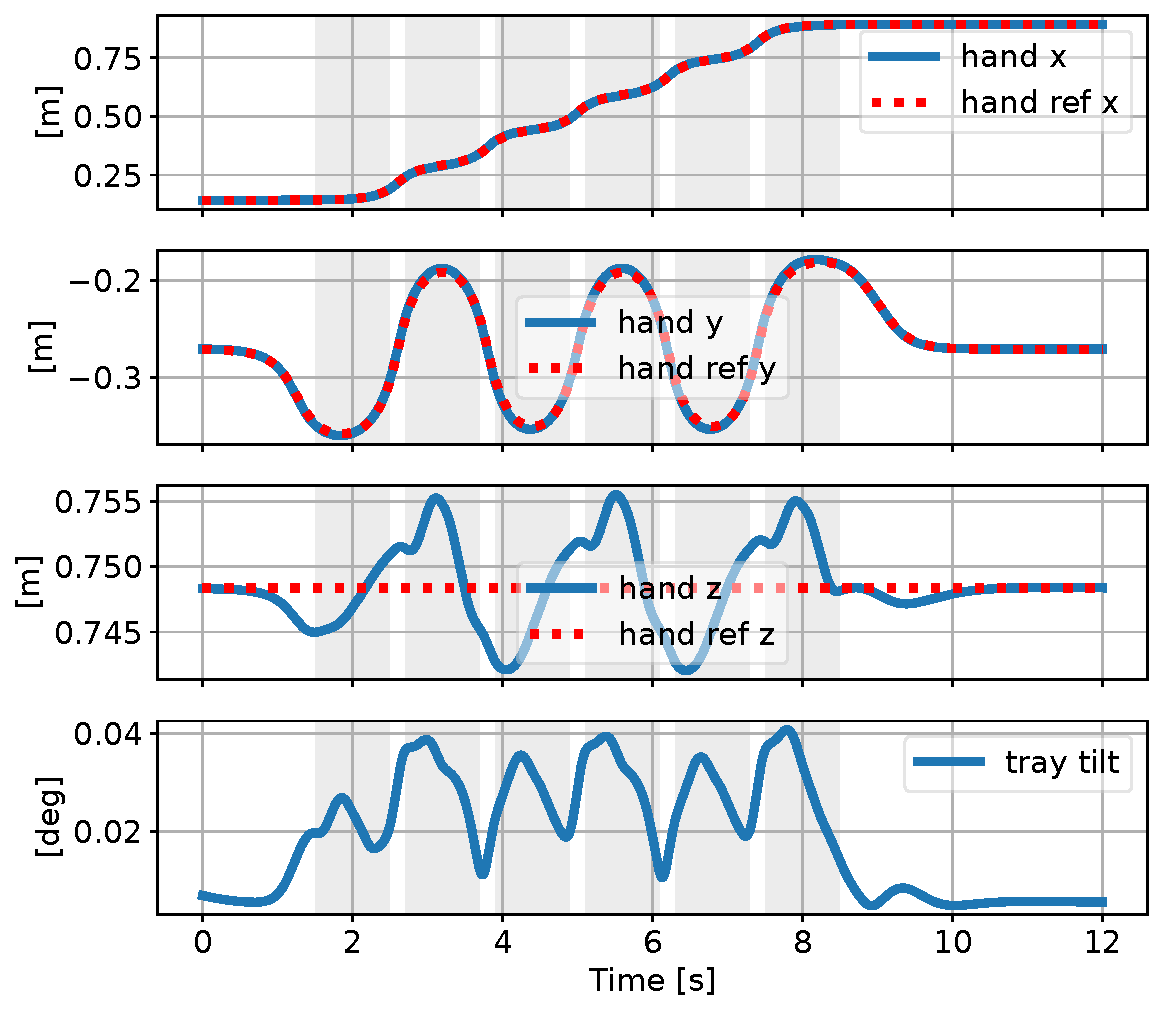
\includegraphics[width=\linewidth]{q3_whand1_hand}\caption{\code{w\_hand} = 1}\end{subfigure}
  \caption{Q3, Hand position and reference, and tray tilt, without and with the tray task.}\label{fig:q3hand}
\end{figure}

\begin{figure}[p]\centering
  \begin{subfigure}{0.49\linewidth}\centering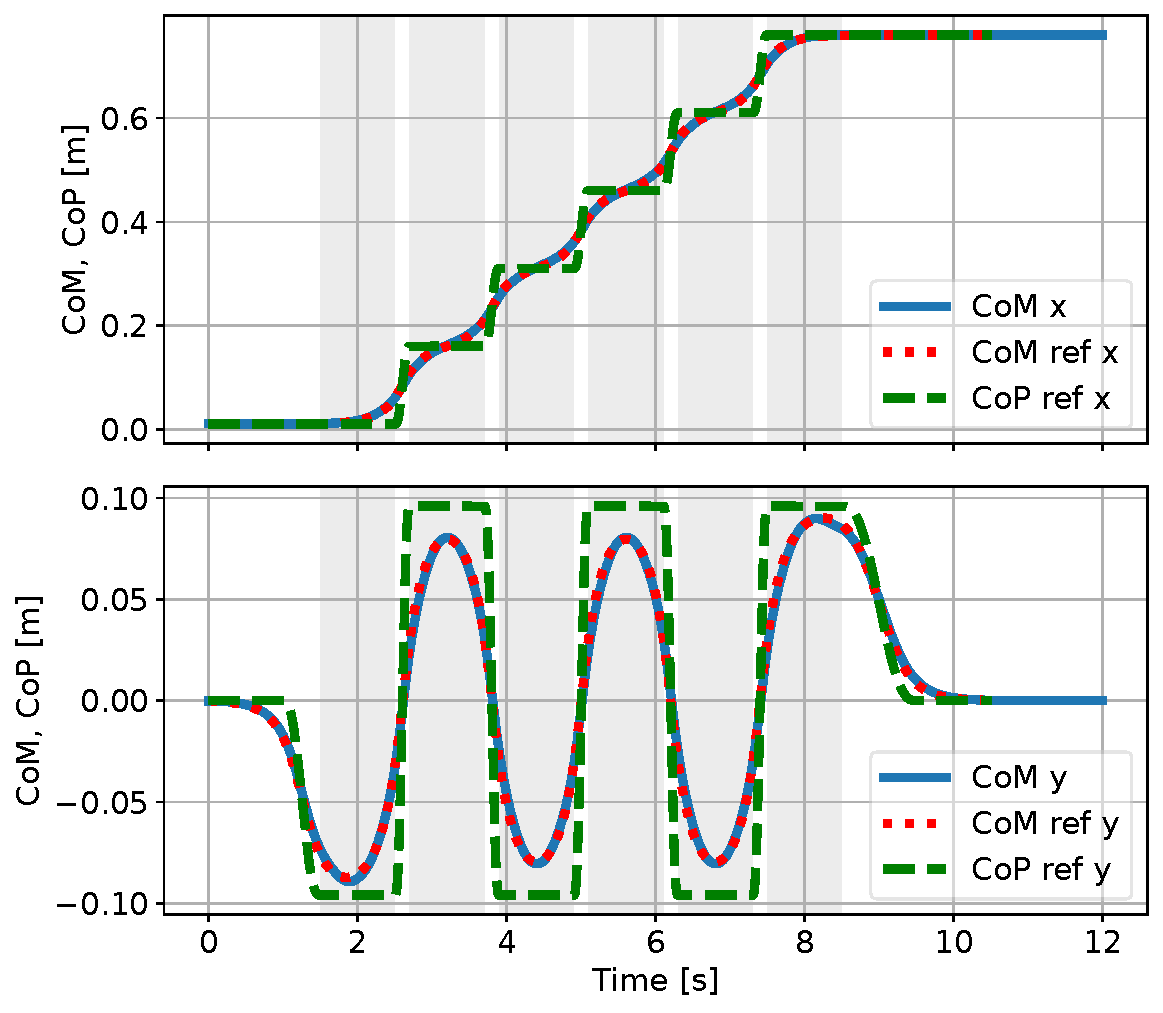
\includegraphics[width=\linewidth]{q3_whand0_com}\caption{\code{w\_hand} = 0}\end{subfigure}
  \hfill
  \begin{subfigure}{0.49\linewidth}\centering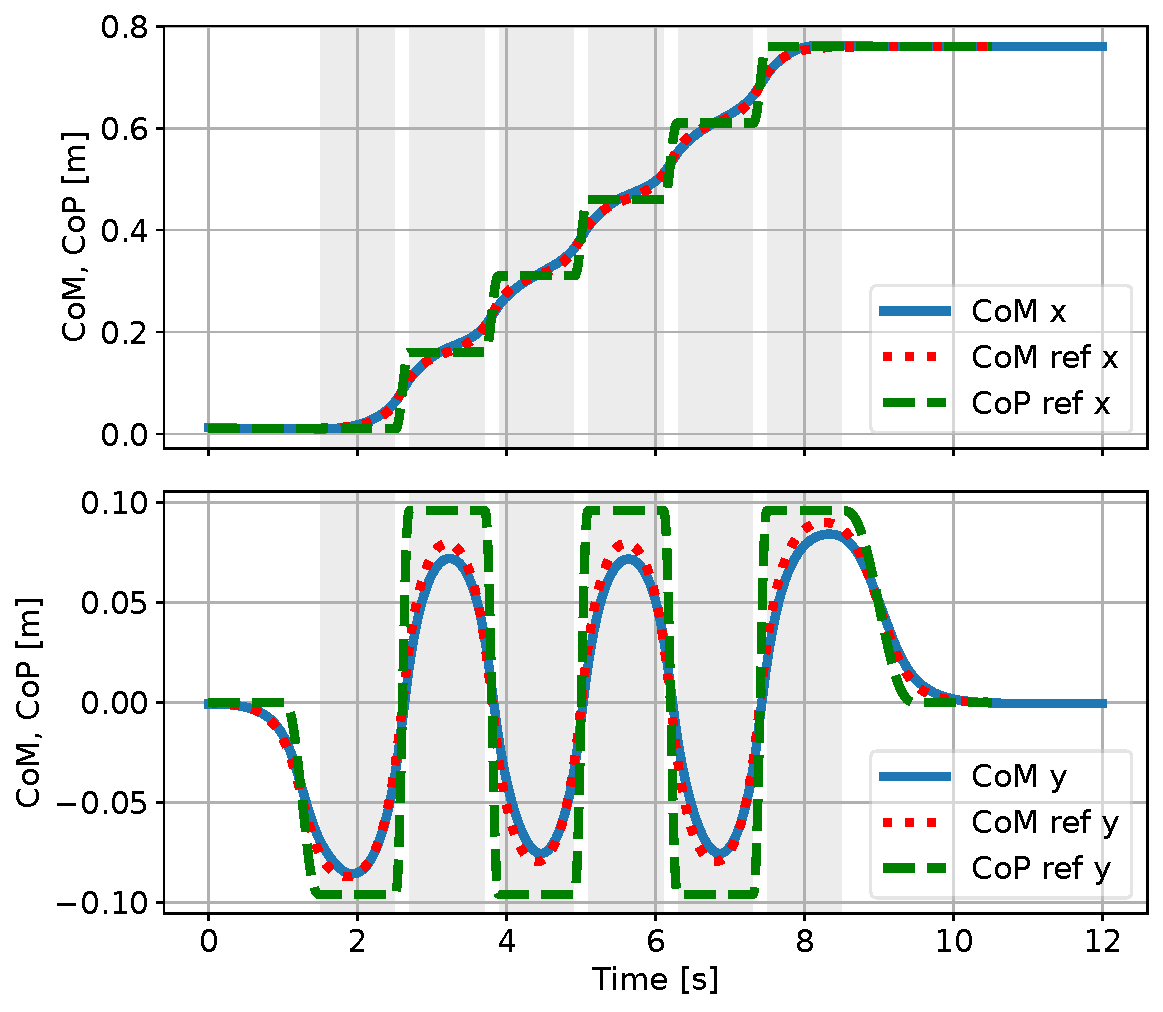
\includegraphics[width=\linewidth]{q3_whand1_com}\caption{\code{w\_hand} = 1}\end{subfigure}
  \caption{Q3, CoM and CoM reference without and with the tray task.}\label{fig:q3com}
\end{figure}

\begin{figure}[p]\centering
  \begin{subfigure}{0.49\linewidth}\centering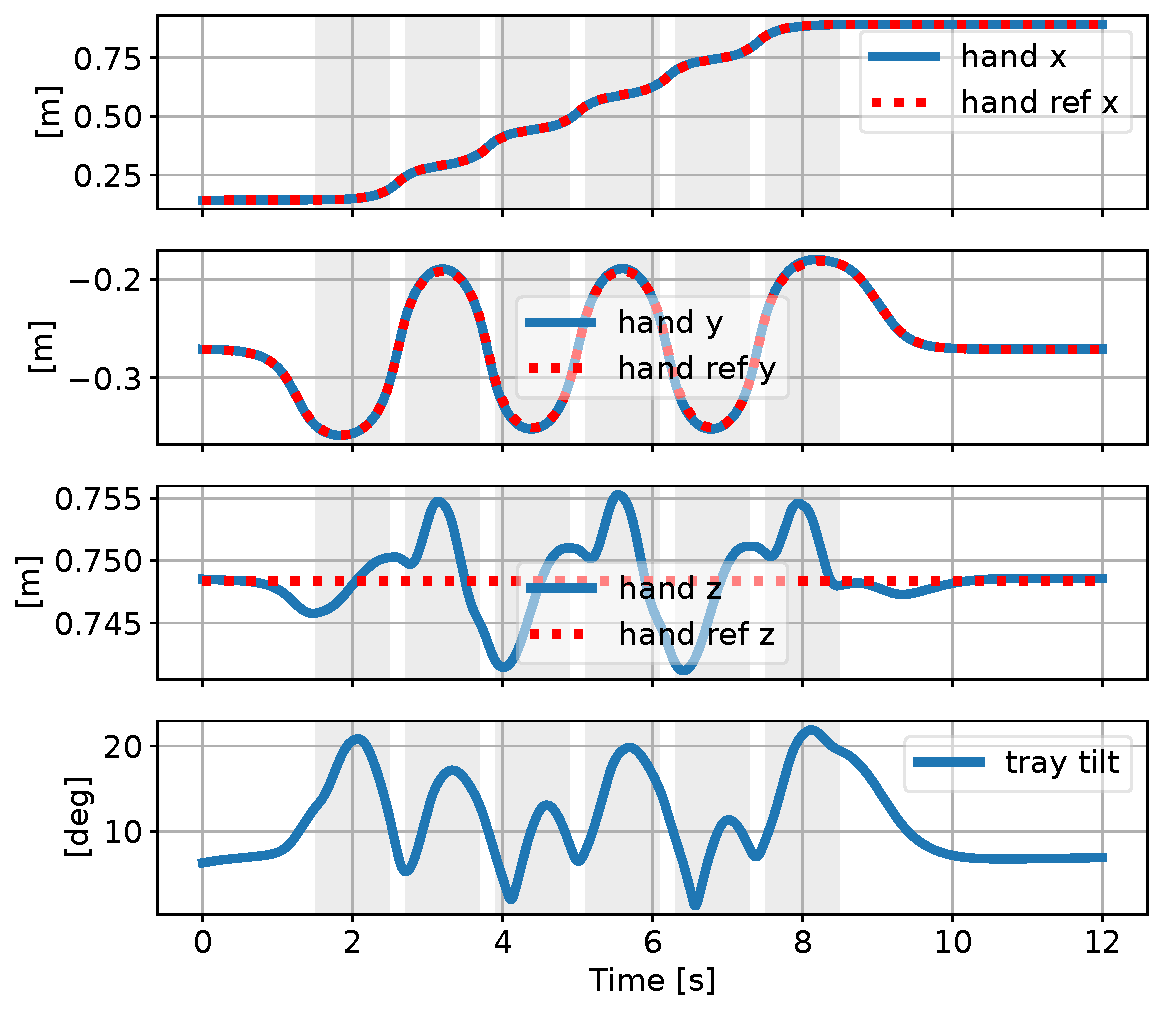
\includegraphics[width=\linewidth]{q4_position_local_hand}\caption{Position only $[1,1,1,0,0,0]$, local frame}\end{subfigure}
  \hfill
  \begin{subfigure}{0.49\linewidth}\centering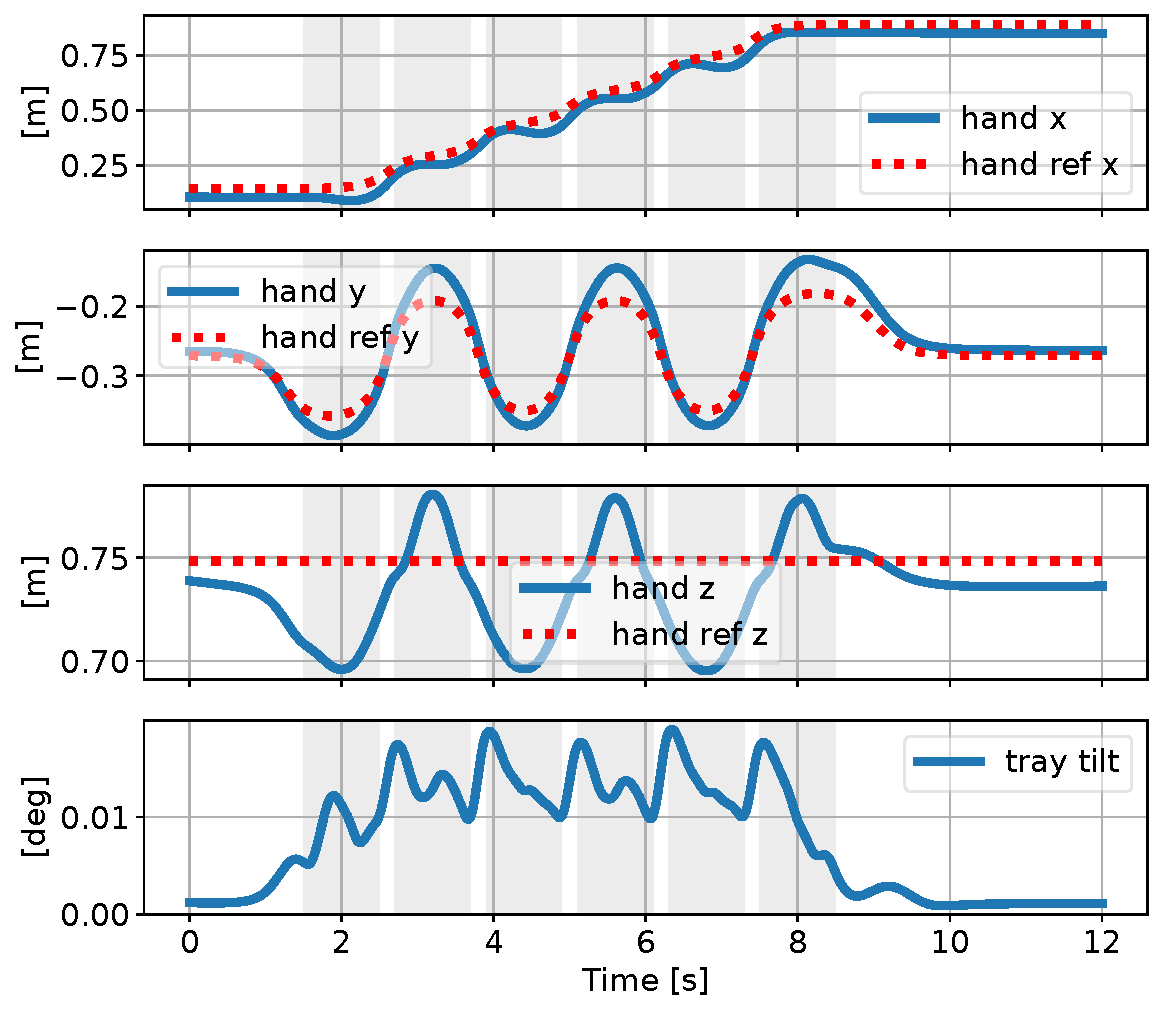
\includegraphics[width=\linewidth]{q4_attitude_local_hand}\caption{Attitude only $[0,0,0,1,1,1]$, local frame}\end{subfigure}
  \medskip
  \begin{subfigure}{0.49\linewidth}\centering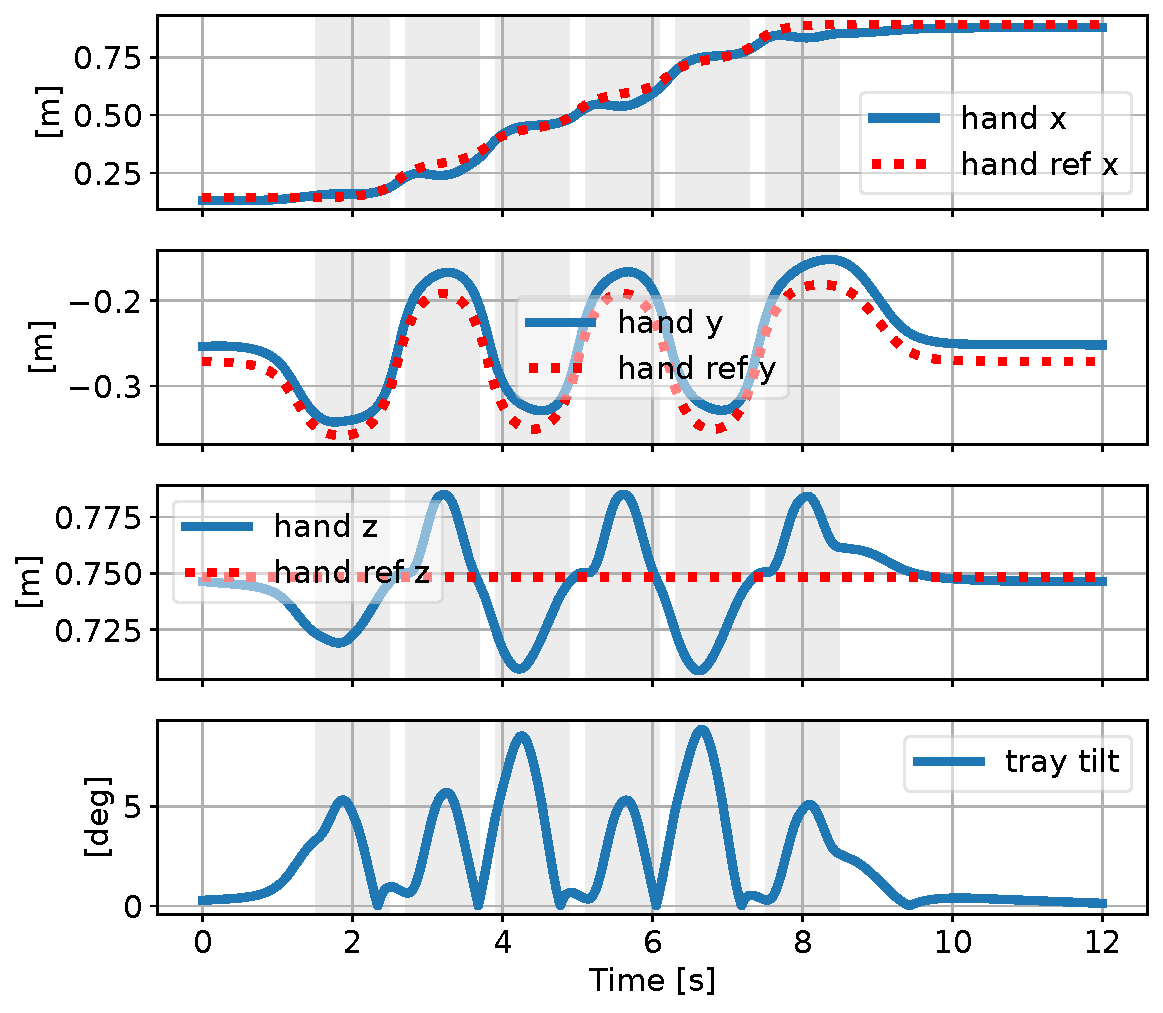
\includegraphics[width=\linewidth]{q4_waiter_local_hand}\caption{Waiter $[0,0,1,1,1,0]$, local frame}\end{subfigure}
  \hfill
  \begin{subfigure}{0.49\linewidth}\centering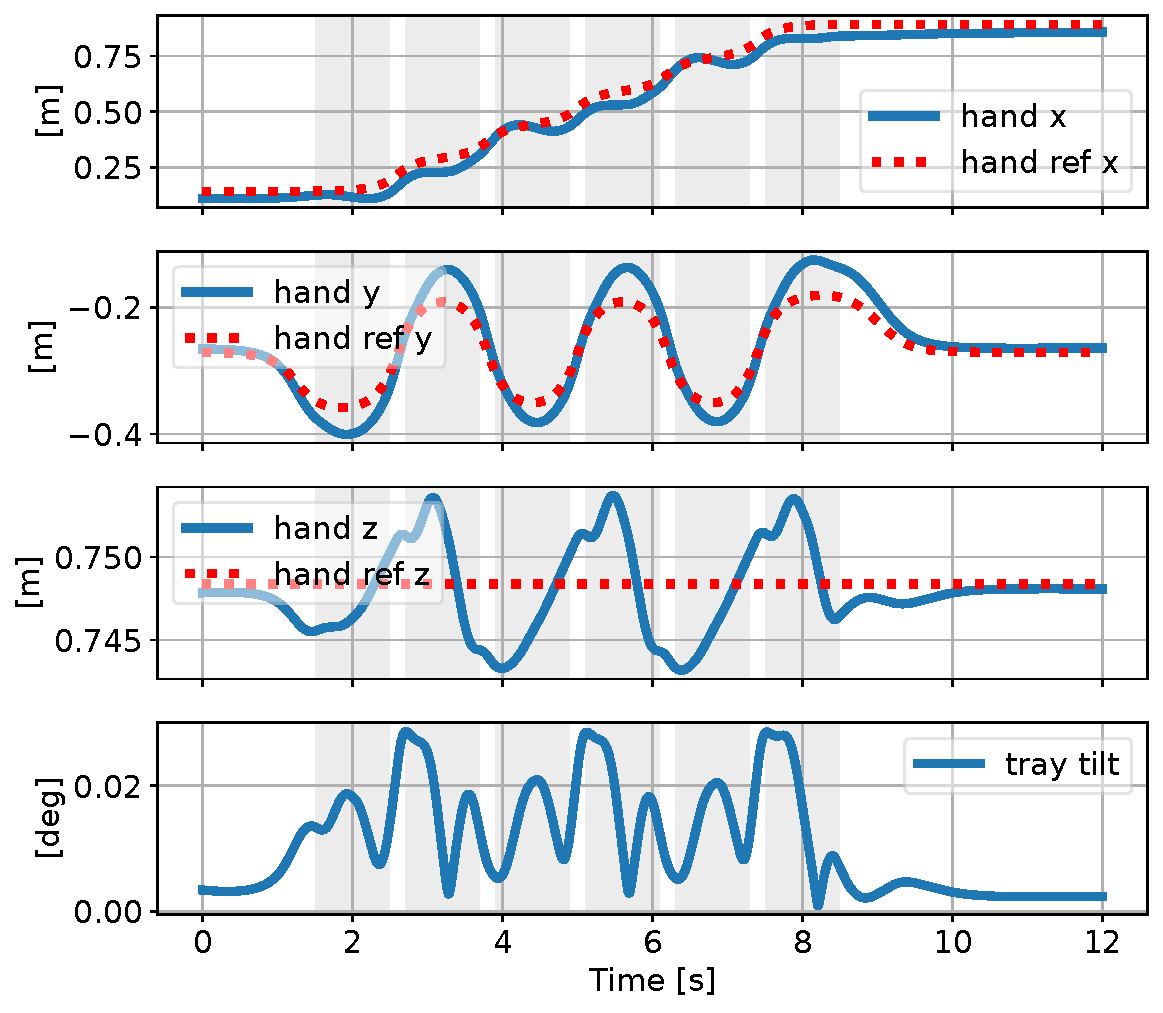
\includegraphics[width=\linewidth]{q4_waiter_world_hand}\caption{Waiter $[0,0,1,1,1,0]$, world frame}\end{subfigure}
  \caption{Q4, Hand position and reference, and tray tilt, for the different masks and frames.}\label{fig:q4time}
\end{figure}

\begin{figure}[p]\centering
  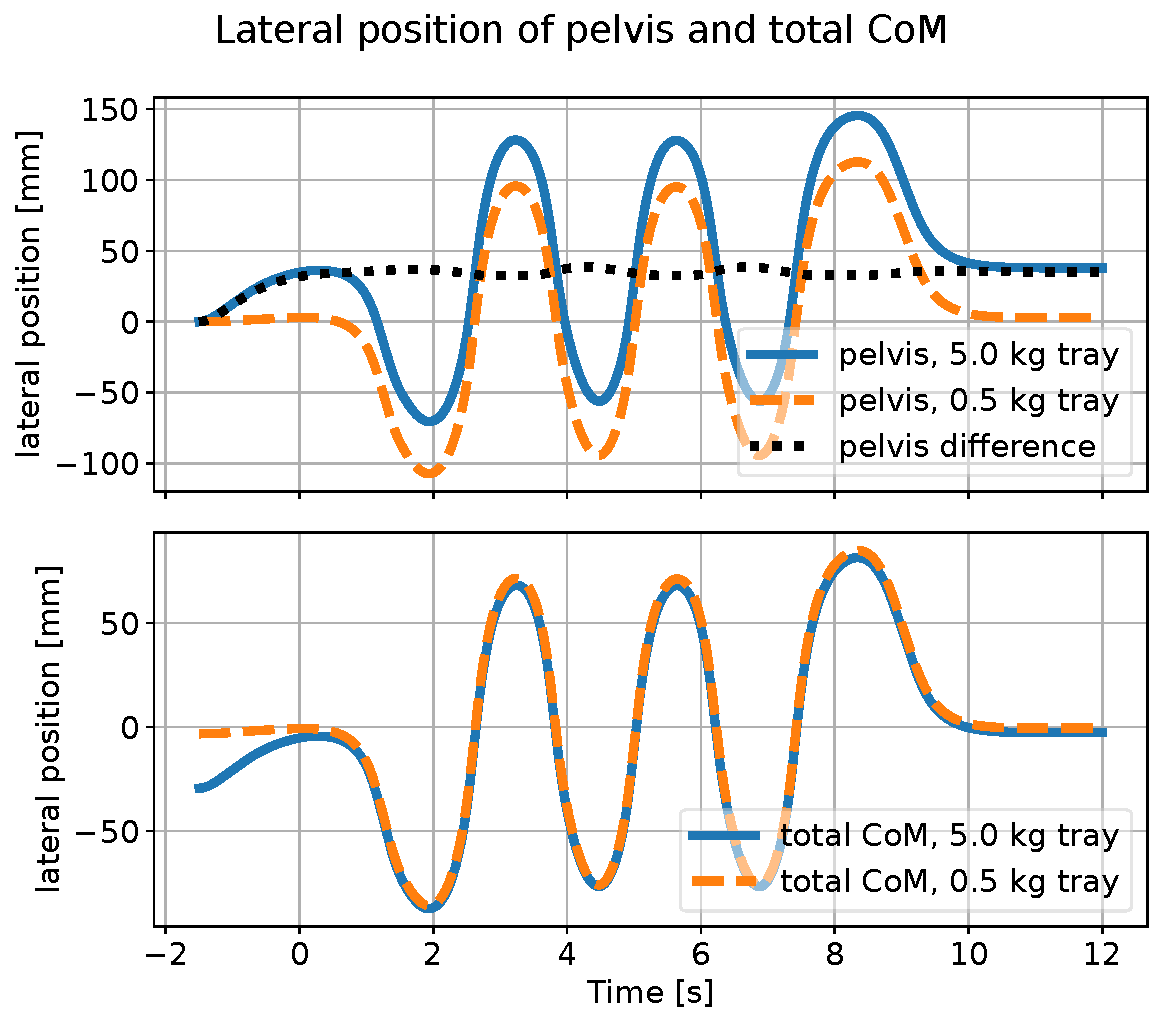
\includegraphics[width=0.6\linewidth]{q5_payloads_lateral}
  \caption{Q5, Lateral position of the pelvis and of the total CoM with the 5\,kg tray and the empty tray .}\label{fig:q5pelvis}
\end{figure}

\begin{figure}[p]\centering
  \begin{subfigure}{0.49\linewidth}\centering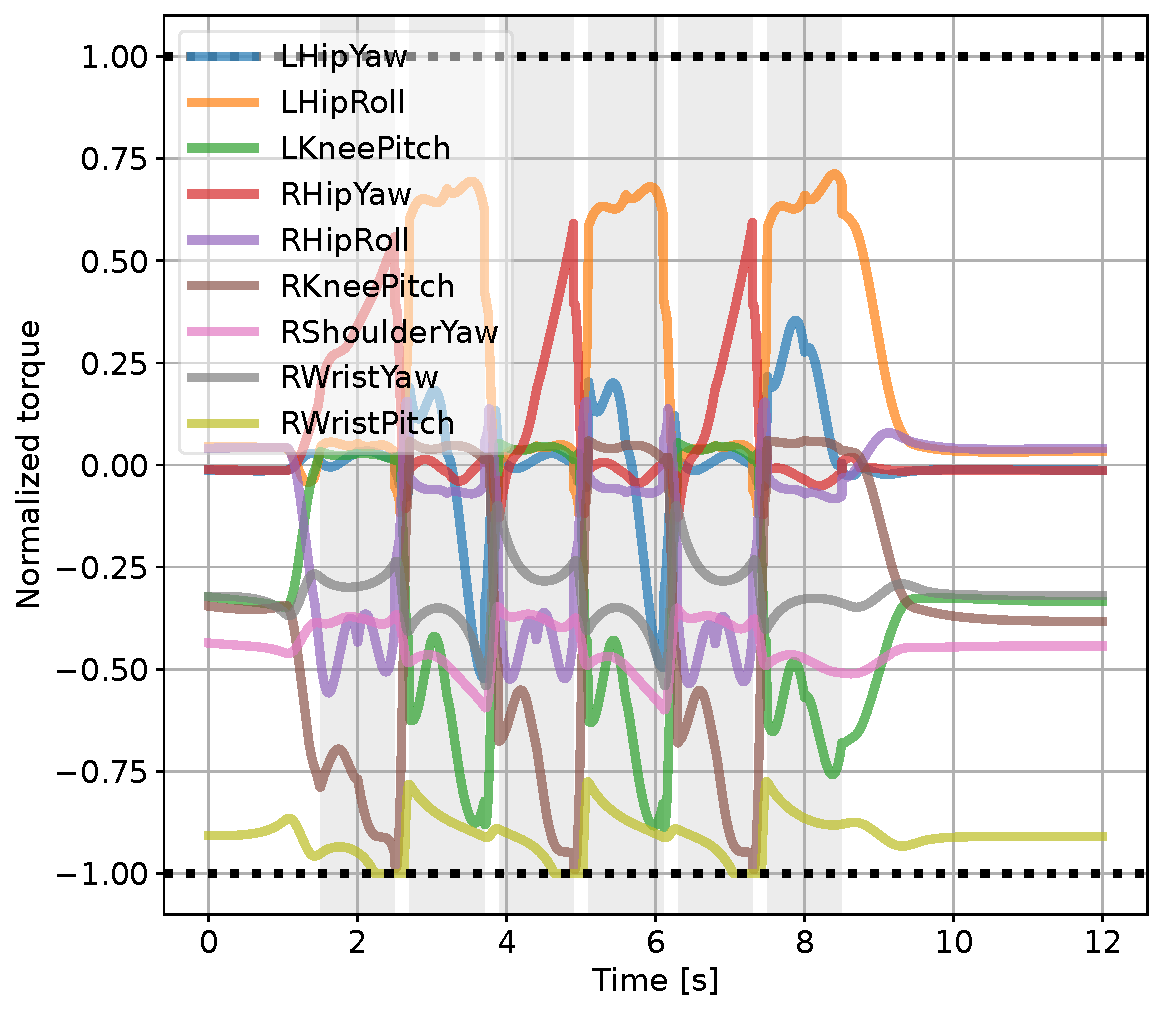
\includegraphics[width=\linewidth]{q5_2kg_weighted_torques}\caption{$w_{hand}=100$}\end{subfigure}
  \hfill
  \begin{subfigure}{0.49\linewidth}\centering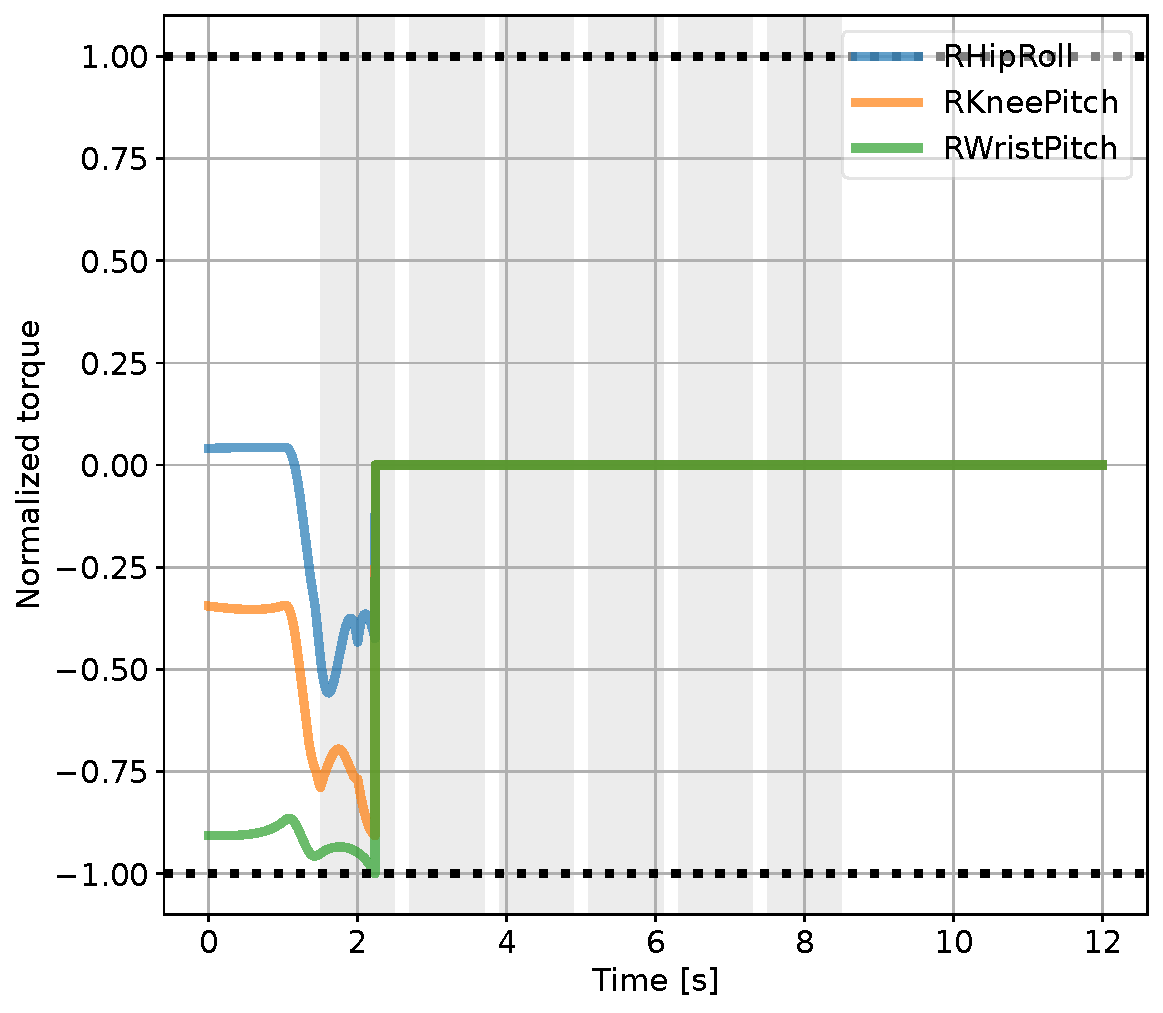
\includegraphics[width=\linewidth]{q5_2kg_hard_torques}\caption{Hard constraint (\code{hand\_priority = 0})}\end{subfigure}
  \caption{Q5, Normalized joint torques with a 2\,kg tray (dotted: limits).}\label{fig:q5tau}
\end{figure}

\begin{figure}[p]\centering
  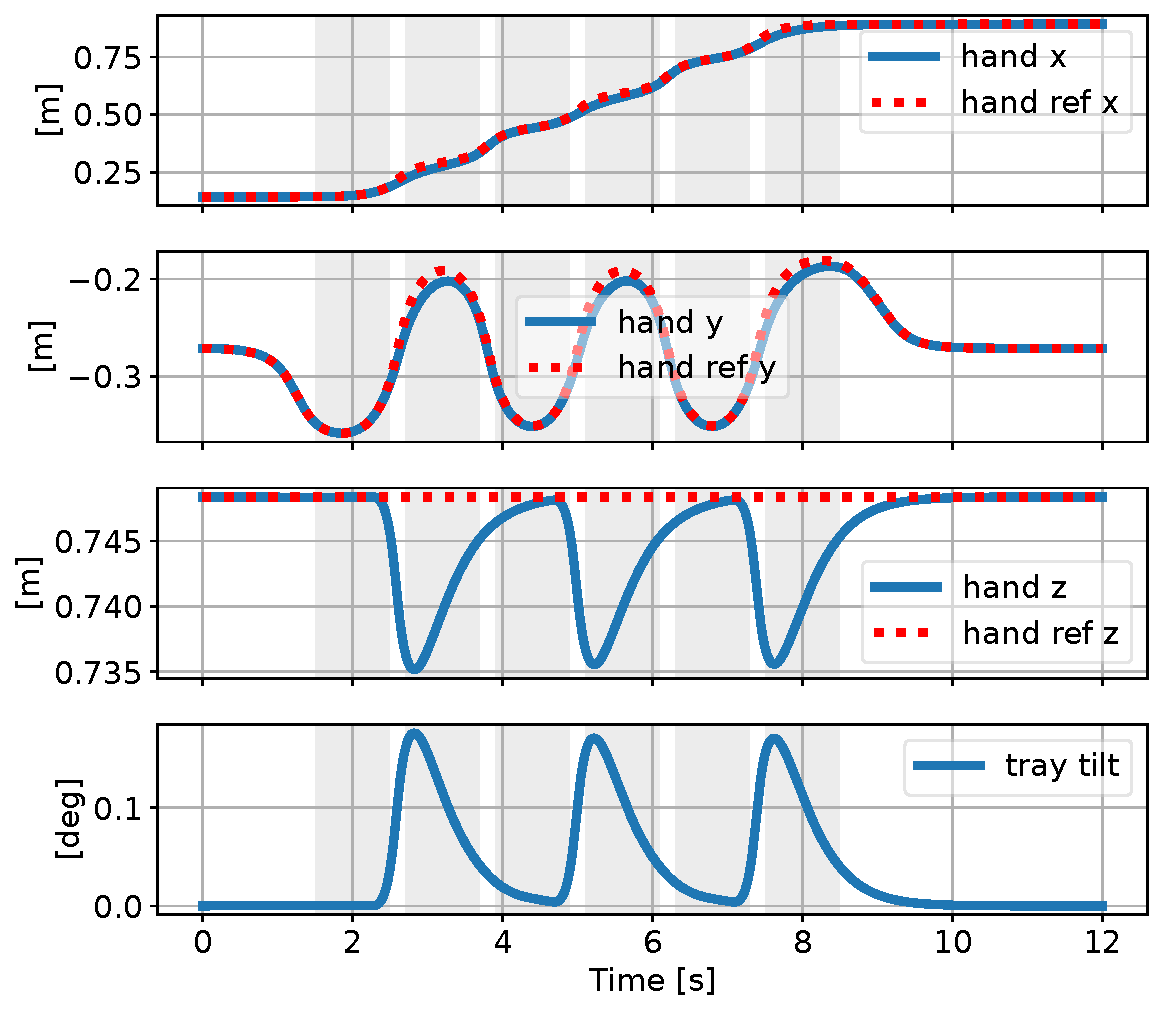
\includegraphics[width=0.6\linewidth]{q5_2kg_weighted_hand}
  \caption{Q5, Hand position and reference, and tray tilt, with a 2\,kg tray and $w_{hand}=100$.}\label{fig:q5tray}
\end{figure}

\end{document}
